% Figure from MATH 591 notes, section 66 (proof that manifolds are paracompact). Added, not from lecture.
% Checked numerically (new/2026-10-26-figcheck/gen.py): the 14 balls cover A_2 and lie in W_2.
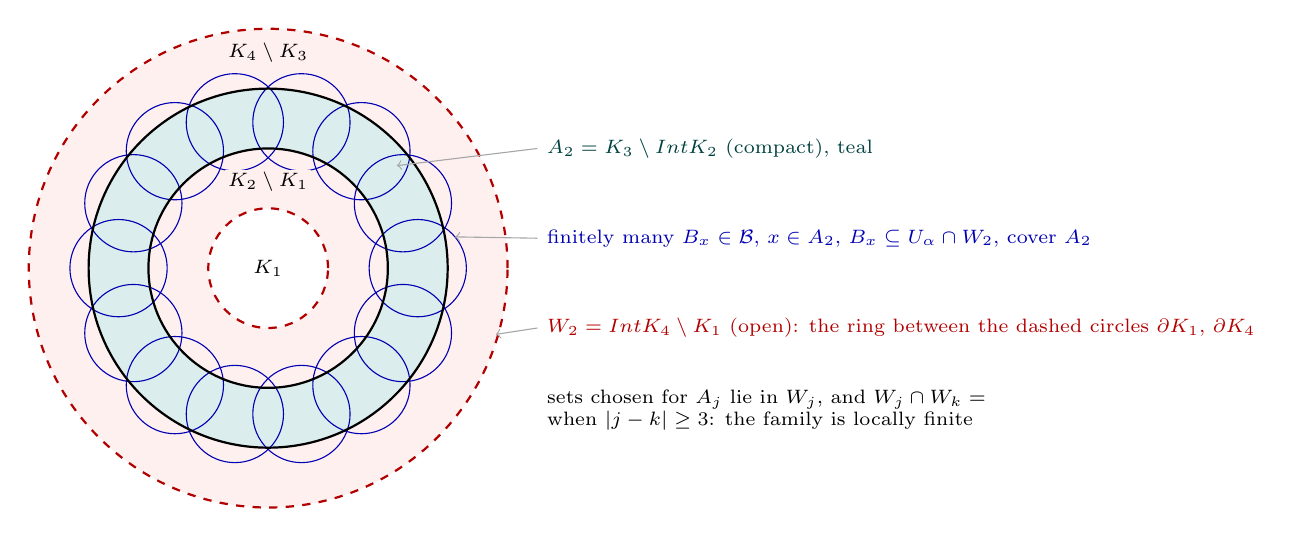
\begin{tikzpicture}[scale=0.95]
    \fill[red!6] (0,0) circle (3.2); \fill[white] (0,0) circle (0.8);
    \fill[teal!14] (0,0) circle (2.4); \fill[red!6] (0,0) circle (1.6);
    \fill[white] (0,0) circle (0.8);
    \foreach \a in {0,25.7143,...,359} { \draw[blue!70!black] ({2.0*cos(\a)},{2.0*sin(\a)}) circle (0.65); }
    \draw[thick] (0,0) circle (1.6) (0,0) circle (2.4);
    \draw[red!70!black, dashed, thick] (0,0) circle (0.8) (0,0) circle (3.2);
    \node[font=\scriptsize] at (0,0) {$K_1$};
    \node[font=\scriptsize, fill=red!6, inner sep=1pt] at (90:1.15) {$K_2 \setminus K_1$};
    \node[font=\scriptsize, fill=red!6, inner sep=1pt] at (90:2.88) {$K_4 \setminus K_3$};
    \draw[->, gray!70] (3.6,1.6) node[right, font=\scriptsize, teal!50!black] {$A_2 = K_3 \setminus \operatorname{Int}K_2$ (compact), teal} -- (1.72,1.37);   % tip at radius 2.2, inside the teal ring
    \draw[->, gray!70] (3.6,0.4) node[right, font=\scriptsize, blue!70!black] {finitely many $B_x \in \mathcal{B}$, $x \in A_2$, $B_x \subseteq U_\alpha \cap W_2$, cover $A_2$} -- (2.498,0.418);
    \draw[->, gray!70] (3.6,-0.8) node[right, font=\scriptsize, red!70!black] {$W_2 = \operatorname{Int}K_4 \setminus K_1$ (open): the ring between the dashed circles $\partial K_1$, $\partial K_4$} -- (3.044,-0.885);
    \node[font=\scriptsize, anchor=west, align=left] at (3.6,-1.9) {sets chosen for $A_j$ lie in $W_j$, and $W_j \cap W_k = \varnothing$\\ when $|j - k| \ge 3$: the family is locally finite};
\end{tikzpicture}
